%!TEX root = Humanoids2013.tex
\section{Simulation Results}
\label{sec:fully_actuated}

Consider some cases of fully actuated and underactuated systems by simulations.
%%-%
\begin{figure*}[t]
\centering
\subfigure[Energy saving in terms of $J_1$ for PEAs.]{\label{fig:EnergySaving_J1_PEA}\includegraphics[width=0.5\columnwidth]{dwg/EnergySavingJ1PEA}}
\subfigure[Energy saving in terms of $J_1$ for SEAs.]{\label{fig:EnergySaving_J1_SEA}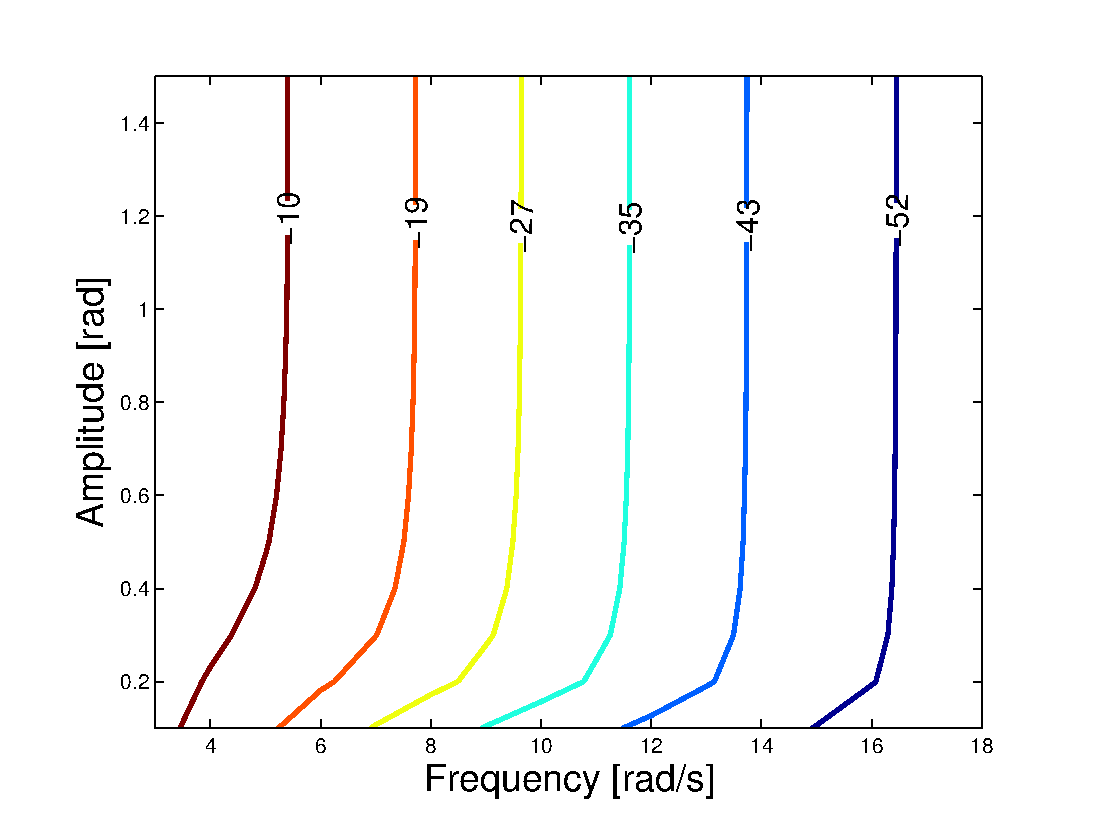
\includegraphics[width=0.5\columnwidth]{dwg/EnergySavingJ1SEA}}
\subfigure[Energy saving in terms of $J_2$ for PEAs.]{\label{fig:EnergySaving_J2_PEA}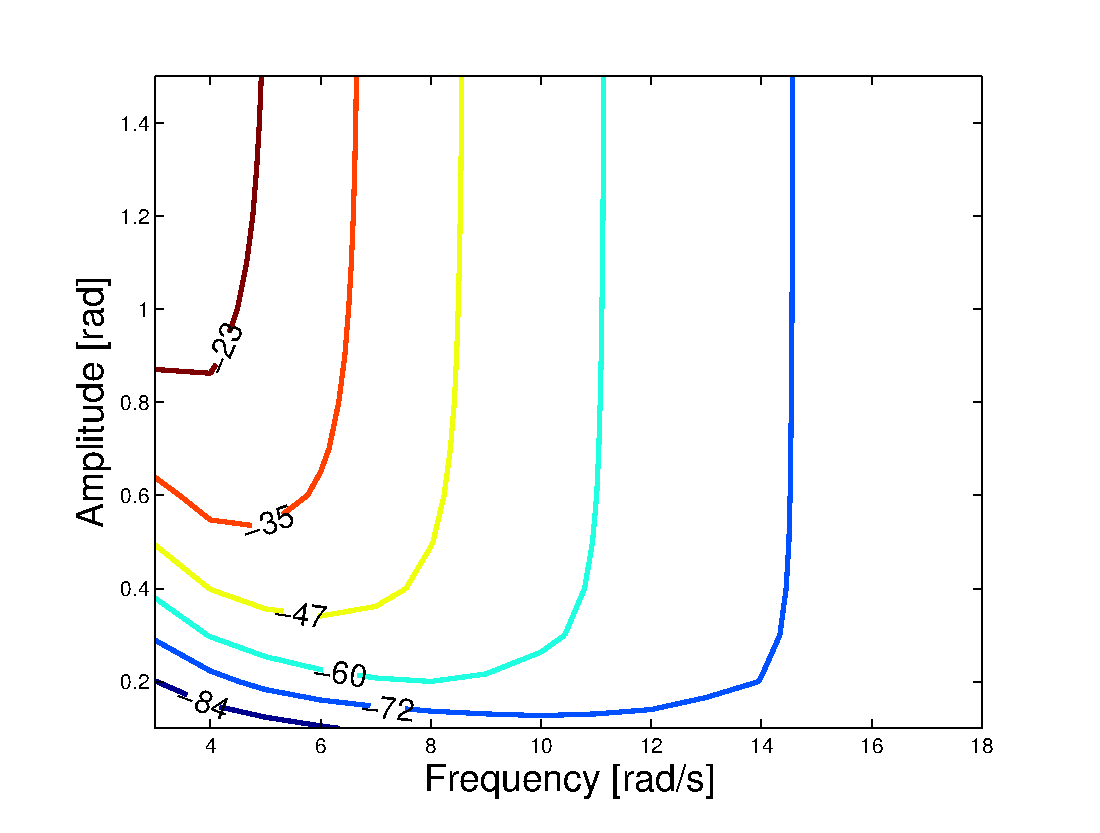
\includegraphics[width=0.5\columnwidth]{dwg/EnergySavingJ2PEA}}
\subfigure[Energy saving in terms of $J_2$ for SEAs.]{\label{fig:EnergySaving_J2_SEA}\includegraphics[width=0.5\columnwidth]{dwg/EnergySavingJ2SEA}}
\caption{Energy saving (in $\%$ w.r.t. the stiff case) for a one-link robot manipulator, varying the amplitude $A$ and the frequency $\omega$ of the desired joint trajectory $q_d(t)=A\sin(\omega t)+B$, with $B=0$.}
\label{fig:EnergySaving}
\end{figure*}

\subsection{One-link Robot manipulator}

First, consider a one-link manipulator, actuated by a SEA or a PEA, which performs a cyclic task. The dynamic of this mechanical system can be written as
\begin{equation}
\begin{aligned}
M\ddot{q} + c\dot{q} + mgL\cos q + K(q-\theta)=0\\
J_{m}\ddot{\theta} + K(\theta-q)=\tau
\end{aligned}
\label{eq:onelinkSEA}
\end{equation}
in case of SEA, and
\begin{equation}
M\ddot{q} + c\dot{q} + mgL\cos q + K(q-q_e)=\tau
\label{eq:onelinkPEA}
\end{equation}
in case of PEA. $M=mL^2+I$, $L$ is the length of the link, $m$ is the load at the end of the link, $I$ the inertia of the link and $c$ is the damping.
Assume that in both cases, the joint trajectory is given as $q_d(t)=B+A\sin(\omega t)$, where the amplitude $A$, the frequency $\omega$, and the angle $B$ around which the link oscillates, depend on the task. 

\paragraph{PEAs} The problem of finding optimal stiffness and pre-load can be solved analytically. Indeed, substituting $q_d(t)$, $\dot q_d(t)$ and $\ddot q_d(t)$ in~\eqref{eq:onelinkPEA}, we can obtain $\tau$
% \[
% \begin{aligned}
% \tau &= A\,M\omega^2\sin(\omega t) + A\,c\,\omega\cos(\omega t) +\\
% &+ mgL\cos(B+A\sin(\omega t)) + K(B+A\sin(\omega t)-q_e)\,.
% \end{aligned}
% \]
and substitute it in $J_1$.
% Let us first consider the cost functional $J_1$ and substitute $\tau$ in it, with $\dot\theta(t)=\dot q(t)$. 
The minimum of $J_1$ is achieved with 
\[
\begin{aligned}
\hat K &= \omega^2 M+\frac{8mgLB_J(2,A)\sin B}{A^2}\\
\hat q_e &= B + \frac{2 g m L A B_J(1,A)\cos B}{A^2\omega^2 M+8mgLB_J(2,A)\sin B}\,,
\end{aligned}
\]
where $B_J(n,x)$ is the Bessel function. Notice that for small amplitudes, i.e.~$A\rightarrow 0$, $\cfrac{8B_J(2,A)}{A^2}\rightarrow 1$, the optimal stiffness becomes $\hat K=\omega^2 M+mgL\sin B$ which corresponds to the resonant condition for the linearized system in $q=B$. % The cost functional in these conditions  becomes
% \begin{equation}
% J_1|_{\hat K,\hat q_e} = A_{PEA}+\pi\frac{A^4 M^2\omega^5-16g^2L^2m^2\omega B_J(1,A)^2}{4}\,.
% \end{equation}
% which is related only on losses due to the damping coefficient.

% Notice that, when $A\rightarrow 0$, i.e. in case of small amplitudes around $q=0$, the optimal stiffness, depending only on $\omega$, does not change whereas the optimal pre-load becomes
% \[
% \hat q_e = \frac{g m L }{\omega^2 M}\,.
% \]
% as the function $\lim_{A\rightarrow 0} B_J(1,\,A)/A=0.5$.
% This result can be obtained considering the linearized system of~\eqref{eq:onelinkPEA} around the point $q=0$ and the optimal stiffness satisfies the resonant condition. As a consequence, the optimal stiffness for the linearized system around $q=0$ is optimal also for the nonlinear system. 

For the cost functional $J_2$, % substituting $q_d(t)$ and its first and second derivative in~\eqref{eq:onelinkPEA}, we have
% \[
% \begin{aligned}
% \tau &= A\,M\omega^2\sin(\omega t) + A\,c\,\omega\cos(\omega t) +\\
% &+ mgL\cos(A\sin(\omega t)) + K(A\sin(\omega t)-q_e)\,.
% \end{aligned}
% \]
% Substituting $\tau$ in the cost functional $J_2$, 
the minimum is obtained with 
\[
\begin{aligned}
\hat K &= \omega^2 M+\frac{2mgLB_J(1,A)\sin B}{A}\\
\hat q_e &= B+\frac{AmgLB_J(0,A)\cos B}{A^2\omega^2 M+2mgLB_J(1,A)\sin B}\,.
\end{aligned}
\]
Also in this case, for small amplitudes, the optimal stiffness becomes $\hat K=\omega^2 M+mgL\sin B$ which corresponds to the resonant condition for the linearized system in $q=B$. % Under these conditions the cost functional can be then rewritten as
% \begin{equation}
% J_2|_{\hat K,\hat q_e} = \pi A^2 c^2 \omega\,,
% \end{equation}
% which is related only to the losses due to the damping coefficient. 
Of course, for the nonlinear system, the cost function obtained by using the optimal parameters assumes a bigger value but $|\tau|$ achieves the minimum value. This is similar to the resonance concept of linear systems.
% This result can be obtained considering the linearized system of~\eqref{eq:onelinkPEA} around the point $q=0$ and the optimal stiffness satisfies the resonant condition. Indeed, this system is a good approximation of the nonlinear one in case of small amplitudes around the origin, i.e.~when $A\rightarrow 0$. Moreover, as the optimal stiffness $K$ obtained for the nonlinear system, depending only on $\omega$, is also optimal for the linearized one, the optimal pre-load value depends also on the amplitude $A$ and for the linearized system becomes 
% \[
% \hat q_e = \frac{g m L}{\omega^2 M}
% \]
% as $\lim_{A\rightarrow 0}B_J(0,A)=1$. 

Finally, for a given $B$, the optimal values for $\hat K$ obtained by using $J_1$ and $J_2$ are quite similar. In particular, if $B=0$ and for any amplitude $A$, $\hat K=\omega^2 M$, i.e.~the value of stiffness corresponding to the resonant condition for the linearized system in $q=0$. The pre-load are different but from a quantitative point of view are quite similar, depending mainly on $B$.

\paragraph{SEAs} The problem of finding optimal stiffness can be solved analytically only in case of $J_2$ as cost functional. Indeed, solving the first equation of \eqref{eq:onelinkSEA} for $\theta$ and substituting it, with its second derivative in the second equation of \eqref{eq:onelinkSEA}, we obtain $\tau$
% \[
% \begin{aligned}
% \tau &= \frac{1}{K}(-A^2 m g L J_m \omega^2 \cos^2(\omega t)\cos(A \sin(\omega t)+B)+\\
% &+A \omega^2 \sin(\omega t) (m g L J_m \sin(A sin(\omega t)+B)+\\
% &-K (M+J_m)+M J_m \omega^2)+ K m g L \cos(A \sin(\omega t)+B)+\\
% &+A d \omega (K-J_m \omega^2) \cos(\omega t))\,.
% \end{aligned}
% \]
and substituting it in $J_2$, with $\dot\theta(t)=K^{-1}(M\ddot q_d(t)+c\,\dot q_d(t)+mgL\cos q_d(t))+q_d(t)$, the minimum can be achieved in closed form. The expression is complicated and can not be reported here. However, in case of $B=0$, $d=0$ and for small amplitudes, the optimal value is
\[
\begin{aligned}
\hat K &= \frac{MJ_m\omega^2}{(M+J_m)}\,,
\end{aligned}
\]
which corresponds to resonant condition for the linearized system around $q=0$, without losses ($d=0$). 

In case of $J_1$, the optimal stiffness and the corresponding value of the cost functional can be only obtained numerically. 
For a comparison between PEA and SEA in terms of efficiency, and to underline the advantage of soft w.r.t.~stiff actuation, in Fig.~\ref{fig:EnergySaving} we report the cost saving in terms of $J_1$ and $J_2$ in case of PEAs or SEAs w.r.t. the stiff case. In particular, Fig.~\ref{fig:EnergySaving_J1_PEA} and \ref{fig:EnergySaving_J1_SEA} show the energy saving using $J_1$ as measure. On the other hand, Fig.~\ref{fig:EnergySaving_J2_PEA} and \ref{fig:EnergySaving_J2_SEA} show the energy saving using $J_2$ as measure.

In particular, considering Fig.~\ref{fig:EnergySaving_J1_PEA} and \ref{fig:EnergySaving_J2_PEA}, the use of PEAs permit to get as much more saving as the amplitude and the frequency of the desired trajectory decrease, independently from the cost functional used, i.e.~$J_1$ or $J_2$. However, we have a consistent saving also in case of large values of frequency, independently from the amplitude. 

Differently, in case of SEA, savings depend on the cost functional we consider. In terms of $J_1$, consistent savings can be obtained increasing the frequency. The amplitude significantly influence only for small values. In terms of $J_2$, consistent savings can be obtained for small values of the amplitude and large values of frequency or for large values of the amplitude and small values of frequency. 

From another point of view, we can conclude that, in terms of $J_2$, PEA is more convenient for small amplitudes at low frequency or large amplitudes at high frequency, while SEA is more convenient for small amplitudes at high frequency or for large amplitudes at low frequency. In terms of $J_1$, we can observe differences w.r.t. $J_2$ only in case of SEA. Indeed, SEA becomes convenient only for high frequencies, independently from the amplitude.
% \begin{figure}[!t]
% \centering
% 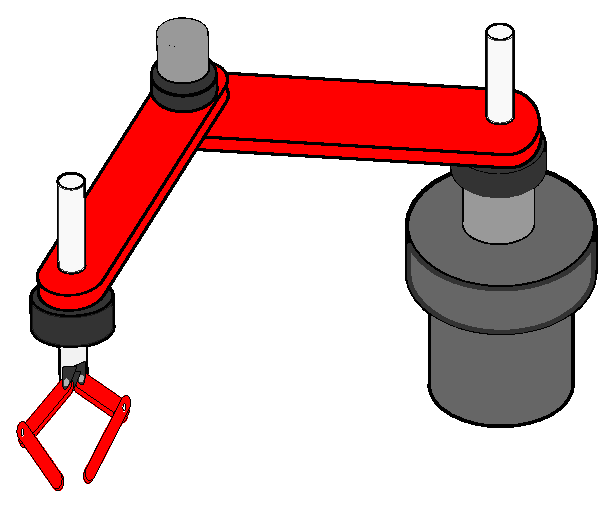
\includegraphics[width=0.6\columnwidth]{dwg/scara}
% \caption{Two-DoF robot Manipulator for a pick and place task.}
% % With, $m = 0.840 \ [kg]; \ l_1 = 0.140 \ [m]; \ l_2 = 0.165 \ [m]; \ l = 0.055 \ [m]$
% \label{fig:scara}
% \end{figure}
%%-%
\begin{figure*}[!t]
\centering
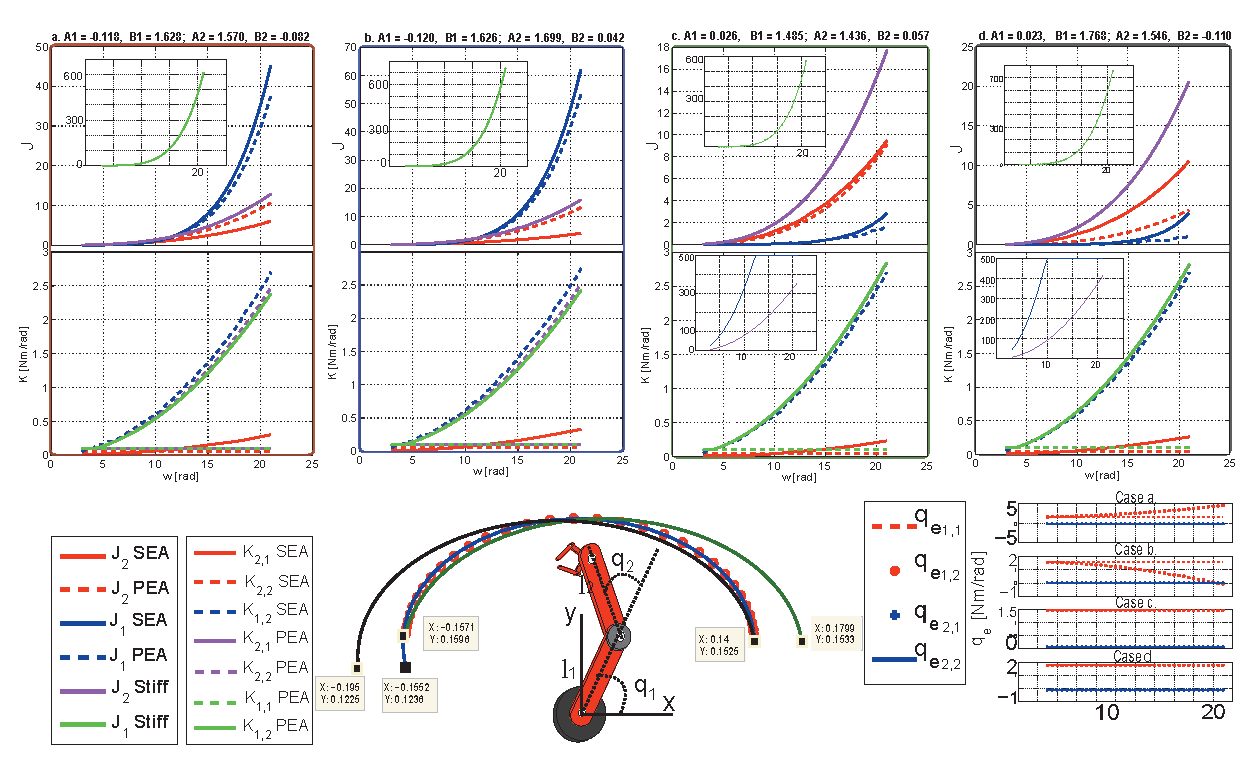
\includegraphics[width=0.88\textwidth]{dwg/TwoLinksManipulator}
\caption{The dynamics parameters used are: link masses $m_1 = m_2 = 0.84$~kg; link lengths $l_1 = 0.14$~m, $l_2 = 0.165$~m; motor inertias $J_{m_{1}} = J_{m_{2}} = 10^{-5}$~$kg m^2$, link inertias motor inertias $J_1 = 3.96\,10^{-4}$~kgm$^2$ $J_2 = 5.29\,10^{-4}$~kgm$^2$ w.r.t. centroid. The red, blue, green and black curves on the center of the figure show the desired end-effector trajectories. The corresponding results of cost functionals and optimal stiffness are shown in the boxes of the same color (a. to d. from left to right). The figure legends are indicated below the boxes. For cases a. and b. (red and blue), $\hat K_{(1,1)SEA} = \ 500 \ Nm/rad$ so it is not shown; for cases c. and d. (green and black) it is indicated with blue continuous line. The pre-load optimization results for the PEA case are shown at bottom right.}
\label{fig:PickAndPlace}
\end{figure*}

\subsection{Two--link robot manipulator}

Let us consider now a two-link robot manipulator which performs a pick and place task. The robot moves on a horizontal plane.
% and hence the dynamic, in case of PEAs, is
% \[
% \dots
% \]
% where $q_1$ and $q_2$ are the link positions, $\ell_1$ and $\ell_2$ the length of each link, $J_1$ and $J_2$ their inertias and $\tau_1$ and $\tau_2$ the torques generated by motors. In case of SEAs, we have
% 
% 
% where $\theta_1$ and $\theta_2$ the motor positions. 
In case of PEAs, we have a fully actuated mechanical system (2 motors and 2 DoFs), whereas in case of SEAs an under-actuated one (2 motors and 4 DoF). $q_{1,d}=A_1\sin(\omega t)+B_1$ and $q_{2,d}=A_2\sin(\omega t)+B_2$ are the desired joint trajectories. The robot moves from a given initial position $Q_1$ to a given final position $Q_2$. The values of the amplitudes $A_1$ and $A_2$, as well as the angle $B_1$ and $B_2$ around which each link moves, depend on these positions. Of course, for any couple of point $Q_1$ and $Q_2$, these parameters are univocally determined by inverse kinematics.
% the desired end-effector trajectory is
% \[
% \begin{aligned}
% 	x_{e,d} &= \ell_1\cos q_{1,d}+\ell_2\cos(q_{1,d}+q_{2,d})\\
% 	y_{e,d} &= \ell_1\sin q_{1,d}+\ell_2\sin(q_{1,d}+q_{2,d})\,,
% \end{aligned}
% \]
% and hence, 
% \[
% \rho_{e,d}=\sqrt{\ell_1^2+\ell_2^2+2\ell_1\ell_2\cos q_{2,d}}
% \]
For this problem, we have performed several simulations applying our methodology. Some of them are reported in Fig.~\ref{fig:PickAndPlace}, which shows the values of cost functionals $J_1$ and $J_2$ in case of PEAs and SEAs, as well as the optimal parameters (stiffness and/or pre-load) for different values of frequency $\omega$. Moreover, cost functionals $J_1$ and $J_2$ for the same tasks for the stiff case are also reported. Notice that for all cases reported in Figure~\ref{fig:PickAndPlace}, the cost functionals assume the minimum values. % and $A_1\equiv A_2$.

For all cases, it is shown in Fig.~\ref{fig:PickAndPlace} that the stiff actuation is the most expensive in terms of energy spent. Furthermore, in the first two cases (a. and b.), when using $J_1$, PEA gives the lowest cost, while for the other two cases (c. and d.) the best performance is achieved when using SEA. The same happens for $J_2$. The optimal joint stiffness is higher as $\omega$ increases.
Moreover, for the SEA case, the spring in the first joint should be stiffer than the second joint, while for the PEA case, the spring for the first joint should be softer than the second one. Results evidence that elastic actuators allow to save energy. Indeed, at the highest frequency used in these simulations, the energy savings in terms of cost functional $J_1$ is up to $90\%$ w.r.t.~the rigid case in the SEA and PEA cases. In terms of $J_2$, at the same frequency, the energy savings is up to $62\%$ in case of SEAs and $23\%$ in case of PEAs, w.r.t.~the rigid case. In Fig.~\ref{fig:PickAndPlace} is also reported values of the optimal pre-load values $q_e$ for the PEA case. Notice that this value is constant for all cases except for the cases a. and b. where the optimal pre-load value of the second joint changes with frequency.

% For all cases, it is shown in Figure~\ref{fig:PickAndPlace} that using $J_1$, the stiff actuation is the most expensive in terms of energy spent, as well as when using $J_2$. Furthermore, for both indices $J_1$ and $J_2$, SEA provides the best performance. For the red and blue curves, and considering the range $\omega \in  \ [3, \ 15]$~rad/s, $J_1$ values in the PEA case are quite similar to those related to the same cost functional but in the SEA case. For higher frequencies, results show that it would be better to use PEA.
% On the other hand, for all cases, the optimal joint stiffness is higher as $\omega$ increases. Moreover, for the SEA case, the first joint should be stiffer than the second joint, while for the PEA case, the first joint should be softer than the second one. Results suggest that in general, elastic actuators allow to save energy; for PEA, $J_2$ is lower, whereas for SEA, $J_1$ has the lowest values. The corresponding joint stiffness are softer than those obtained by using $J_1$ for PEA and $J_2$ for SEA.
